% documentclass: article used for scientific journals, short reports, program documentation, etc
% options: fontsize 11, generate document for double sided printing, a4-paper
\documentclass[11pt, twoside, a4paper]{article}

% package for changing page layout
\usepackage{geometry}
\geometry{a4paper, lmargin=30mm, rmargin=20mm, tmargin=30mm, bmargin=20mm}
% set indentation
\setlength{\parindent}{0mm} 

% input encoding for special characters (e.g. ä,ü,ö,ß), only for non english text
% options: utf8 as encoding standard
\usepackage[utf8]{inputenc}
% package for changing used language
% options: german or default: english
\usepackage[german]{babel}

% package for math symbols, functions and environments from ams(american mathematical society)
\usepackage{amsmath}
% package for extended symbols from ams
\usepackage{amssymb}
% package for extended symbols from stmaryrd(st mary road)
%\usepackage{stmaryrd}
% package for managing pictures
\usepackage{graphicx}

% package for some extra fonts
\usepackage{txfonts}
% package for changing color of font and paper
% options: using names of default colors (e.g red, black)
\usepackage[usenames]{color}

% package for converting eps-files to pdf-files and then include them
\usepackage{epstopdf}
% use another program (ps2pdf) for converting
% !!! important: set shell_escape=1 in /etc/texmf/texmf.cnf (Linux) for allowing to use other programs
% !!!			 or use the command line with -shell-escape
\epstopdfDeclareGraphicsRule{.eps}{pdf}{.pdf}{
ps2pdf -dEPSCrop #1 \OutputFile
}

% package for reference to last page (output number of last page)
\usepackage{lastpage}
% package for using header and footer
% options: automate terms of right and left marks
\usepackage[automark]{scrpage2}
% set style for footer and header
\pagestyle{scrheadings}
% clear pagestyle for redefining
\clearscrheadfoot
% set header and footer: use <xx>head/foot[]{Text} (i...inner, o...outer, c...center, o...odd, e...even, l...left, r...right)
\ihead[]{}
\ohead[]{}
\cfoot[]{\pagemark/\pageref{LastPage}}


% begin the document
\begin{document}
	
	\begin{figure}[h]
		\center
		% GNUPLOT: LaTeX picture with Postscript
\begingroup
  \makeatletter
  \providecommand\color[2][]{%
    \GenericError{(gnuplot) \space\space\space\@spaces}{%
      Package color not loaded in conjunction with
      terminal option `colourtext'%
    }{See the gnuplot documentation for explanation.%
    }{Either use 'blacktext' in gnuplot or load the package
      color.sty in LaTeX.}%
    \renewcommand\color[2][]{}%
  }%
  \providecommand\includegraphics[2][]{%
    \GenericError{(gnuplot) \space\space\space\@spaces}{%
      Package graphicx or graphics not loaded%
    }{See the gnuplot documentation for explanation.%
    }{The gnuplot epslatex terminal needs graphicx.sty or graphics.sty.}%
    \renewcommand\includegraphics[2][]{}%
  }%
  \providecommand\rotatebox[2]{#2}%
  \@ifundefined{ifGPcolor}{%
    \newif\ifGPcolor
    \GPcolorfalse
  }{}%
  \@ifundefined{ifGPblacktext}{%
    \newif\ifGPblacktext
    \GPblacktexttrue
  }{}%
  % define a \g@addto@macro without @ in the name:
  \let\gplgaddtomacro\g@addto@macro
  % define empty templates for all commands taking text:
  \gdef\gplbacktext{}%
  \gdef\gplfronttext{}%
  \makeatother
  \ifGPblacktext
    % no textcolor at all
    \def\colorrgb#1{}%
    \def\colorgray#1{}%
  \else
    % gray or color?
    \ifGPcolor
      \def\colorrgb#1{\color[rgb]{#1}}%
      \def\colorgray#1{\color[gray]{#1}}%
      \expandafter\def\csname LTw\endcsname{\color{white}}%
      \expandafter\def\csname LTb\endcsname{\color{black}}%
      \expandafter\def\csname LTa\endcsname{\color{black}}%
      \expandafter\def\csname LT0\endcsname{\color[rgb]{1,0,0}}%
      \expandafter\def\csname LT1\endcsname{\color[rgb]{0,1,0}}%
      \expandafter\def\csname LT2\endcsname{\color[rgb]{0,0,1}}%
      \expandafter\def\csname LT3\endcsname{\color[rgb]{1,0,1}}%
      \expandafter\def\csname LT4\endcsname{\color[rgb]{0,1,1}}%
      \expandafter\def\csname LT5\endcsname{\color[rgb]{1,1,0}}%
      \expandafter\def\csname LT6\endcsname{\color[rgb]{0,0,0}}%
      \expandafter\def\csname LT7\endcsname{\color[rgb]{1,0.3,0}}%
      \expandafter\def\csname LT8\endcsname{\color[rgb]{0.5,0.5,0.5}}%
    \else
      % gray
      \def\colorrgb#1{\color{black}}%
      \def\colorgray#1{\color[gray]{#1}}%
      \expandafter\def\csname LTw\endcsname{\color{white}}%
      \expandafter\def\csname LTb\endcsname{\color{black}}%
      \expandafter\def\csname LTa\endcsname{\color{black}}%
      \expandafter\def\csname LT0\endcsname{\color{black}}%
      \expandafter\def\csname LT1\endcsname{\color{black}}%
      \expandafter\def\csname LT2\endcsname{\color{black}}%
      \expandafter\def\csname LT3\endcsname{\color{black}}%
      \expandafter\def\csname LT4\endcsname{\color{black}}%
      \expandafter\def\csname LT5\endcsname{\color{black}}%
      \expandafter\def\csname LT6\endcsname{\color{black}}%
      \expandafter\def\csname LT7\endcsname{\color{black}}%
      \expandafter\def\csname LT8\endcsname{\color{black}}%
    \fi
  \fi
  \setlength{\unitlength}{0.0500bp}%
  \begin{picture}(8502.00,5102.00)%
    \gplgaddtomacro\gplbacktext{%
      \csname LTb\endcsname%
      \put(1078,704){\makebox(0,0)[r]{\strut{} 100}}%
      \put(1078,1078){\makebox(0,0)[r]{\strut{} 200}}%
      \put(1078,1451){\makebox(0,0)[r]{\strut{} 300}}%
      \put(1078,1825){\makebox(0,0)[r]{\strut{} 400}}%
      \put(1078,2199){\makebox(0,0)[r]{\strut{} 500}}%
      \put(1078,2573){\makebox(0,0)[r]{\strut{} 600}}%
      \put(1078,2946){\makebox(0,0)[r]{\strut{} 700}}%
      \put(1078,3320){\makebox(0,0)[r]{\strut{} 800}}%
      \put(1078,3694){\makebox(0,0)[r]{\strut{} 900}}%
      \put(1078,4067){\makebox(0,0)[r]{\strut{} 1000}}%
      \put(1078,4441){\makebox(0,0)[r]{\strut{} 1100}}%
      \put(1210,484){\makebox(0,0){\strut{} 25}}%
      \put(1900,484){\makebox(0,0){\strut{} 30}}%
      \put(2589,484){\makebox(0,0){\strut{} 35}}%
      \put(3279,484){\makebox(0,0){\strut{} 40}}%
      \put(3968,484){\makebox(0,0){\strut{} 45}}%
      \put(4658,484){\makebox(0,0){\strut{} 50}}%
      \put(5347,484){\makebox(0,0){\strut{} 55}}%
      \put(6037,484){\makebox(0,0){\strut{} 60}}%
      \put(6726,484){\makebox(0,0){\strut{} 65}}%
      \put(7416,484){\makebox(0,0){\strut{} 70}}%
      \put(8105,484){\makebox(0,0){\strut{} 75}}%
      \put(176,2572){\rotatebox{-270}{\makebox(0,0){\strut{}$p_D \ [Torr]$}}}%
      \put(4657,154){\makebox(0,0){\strut{}$\vartheta \ [^\circ C]$}}%
      \put(4657,4771){\makebox(0,0){\strut{}Dampfdruckkurve $p_D(\vartheta)$ ohne Korrektur}}%
      \put(1900,2946){\makebox(0,0)[l]{\strut{}$a\pm \Delta a = (6.6 \pm 1.6) \ 10^{8} \ Torr$}}%
      \put(1900,2573){\makebox(0,0)[l]{\strut{}$b\pm \Delta b = (4636 \pm 83) \ K$}}%
    }%
    \gplgaddtomacro\gplfronttext{%
      \csname LTb\endcsname%
      \put(5434,4182){\makebox(0,0)[r]{\strut{}Messwerte ohne Korrektur}}%
      \csname LTb\endcsname%
      \put(5434,3789){\makebox(0,0)[r]{\strut{}$f(x) = a \exp \left(\dfrac{-b}{x+273.15 \ K}\right )$}}%
    }%
    \gplbacktext
    \put(0,0){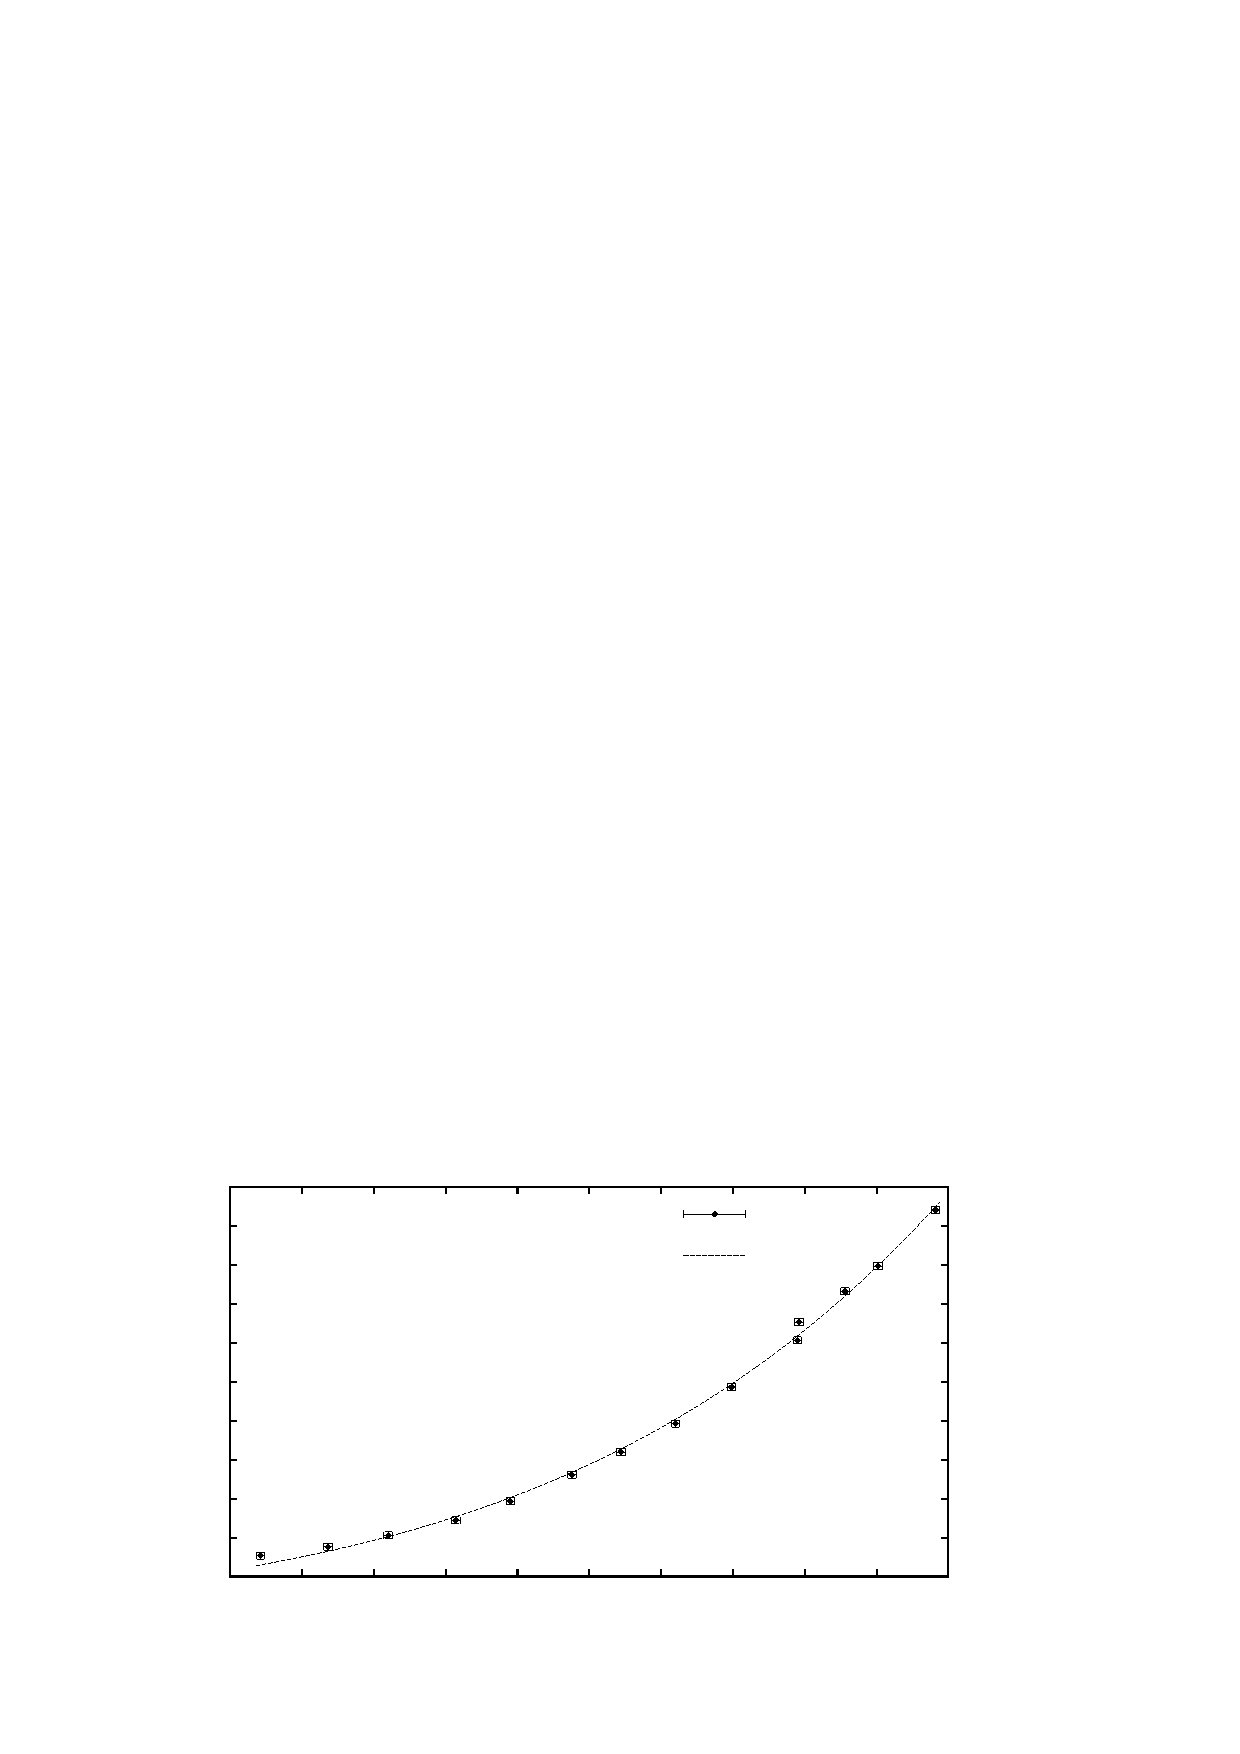
\includegraphics{pD-T-diagram}}%
    \gplfronttext
  \end{picture}%
\endgroup

	\end{figure}

	\begin{figure}[h]
		\center
		% GNUPLOT: LaTeX picture with Postscript
\begingroup
  \makeatletter
  \providecommand\color[2][]{%
    \GenericError{(gnuplot) \space\space\space\@spaces}{%
      Package color not loaded in conjunction with
      terminal option `colourtext'%
    }{See the gnuplot documentation for explanation.%
    }{Either use 'blacktext' in gnuplot or load the package
      color.sty in LaTeX.}%
    \renewcommand\color[2][]{}%
  }%
  \providecommand\includegraphics[2][]{%
    \GenericError{(gnuplot) \space\space\space\@spaces}{%
      Package graphicx or graphics not loaded%
    }{See the gnuplot documentation for explanation.%
    }{The gnuplot epslatex terminal needs graphicx.sty or graphics.sty.}%
    \renewcommand\includegraphics[2][]{}%
  }%
  \providecommand\rotatebox[2]{#2}%
  \@ifundefined{ifGPcolor}{%
    \newif\ifGPcolor
    \GPcolorfalse
  }{}%
  \@ifundefined{ifGPblacktext}{%
    \newif\ifGPblacktext
    \GPblacktexttrue
  }{}%
  % define a \g@addto@macro without @ in the name:
  \let\gplgaddtomacro\g@addto@macro
  % define empty templates for all commands taking text:
  \gdef\gplbacktext{}%
  \gdef\gplfronttext{}%
  \makeatother
  \ifGPblacktext
    % no textcolor at all
    \def\colorrgb#1{}%
    \def\colorgray#1{}%
  \else
    % gray or color?
    \ifGPcolor
      \def\colorrgb#1{\color[rgb]{#1}}%
      \def\colorgray#1{\color[gray]{#1}}%
      \expandafter\def\csname LTw\endcsname{\color{white}}%
      \expandafter\def\csname LTb\endcsname{\color{black}}%
      \expandafter\def\csname LTa\endcsname{\color{black}}%
      \expandafter\def\csname LT0\endcsname{\color[rgb]{1,0,0}}%
      \expandafter\def\csname LT1\endcsname{\color[rgb]{0,1,0}}%
      \expandafter\def\csname LT2\endcsname{\color[rgb]{0,0,1}}%
      \expandafter\def\csname LT3\endcsname{\color[rgb]{1,0,1}}%
      \expandafter\def\csname LT4\endcsname{\color[rgb]{0,1,1}}%
      \expandafter\def\csname LT5\endcsname{\color[rgb]{1,1,0}}%
      \expandafter\def\csname LT6\endcsname{\color[rgb]{0,0,0}}%
      \expandafter\def\csname LT7\endcsname{\color[rgb]{1,0.3,0}}%
      \expandafter\def\csname LT8\endcsname{\color[rgb]{0.5,0.5,0.5}}%
    \else
      % gray
      \def\colorrgb#1{\color{black}}%
      \def\colorgray#1{\color[gray]{#1}}%
      \expandafter\def\csname LTw\endcsname{\color{white}}%
      \expandafter\def\csname LTb\endcsname{\color{black}}%
      \expandafter\def\csname LTa\endcsname{\color{black}}%
      \expandafter\def\csname LT0\endcsname{\color{black}}%
      \expandafter\def\csname LT1\endcsname{\color{black}}%
      \expandafter\def\csname LT2\endcsname{\color{black}}%
      \expandafter\def\csname LT3\endcsname{\color{black}}%
      \expandafter\def\csname LT4\endcsname{\color{black}}%
      \expandafter\def\csname LT5\endcsname{\color{black}}%
      \expandafter\def\csname LT6\endcsname{\color{black}}%
      \expandafter\def\csname LT7\endcsname{\color{black}}%
      \expandafter\def\csname LT8\endcsname{\color{black}}%
    \fi
  \fi
  \setlength{\unitlength}{0.0500bp}%
  \begin{picture}(8502.00,5102.00)%
    \gplgaddtomacro\gplbacktext{%
      \csname LTb\endcsname%
      \put(1078,704){\makebox(0,0)[r]{\strut{} 100}}%
      \put(1078,1078){\makebox(0,0)[r]{\strut{} 200}}%
      \put(1078,1451){\makebox(0,0)[r]{\strut{} 300}}%
      \put(1078,1825){\makebox(0,0)[r]{\strut{} 400}}%
      \put(1078,2199){\makebox(0,0)[r]{\strut{} 500}}%
      \put(1078,2573){\makebox(0,0)[r]{\strut{} 600}}%
      \put(1078,2946){\makebox(0,0)[r]{\strut{} 700}}%
      \put(1078,3320){\makebox(0,0)[r]{\strut{} 800}}%
      \put(1078,3694){\makebox(0,0)[r]{\strut{} 900}}%
      \put(1078,4067){\makebox(0,0)[r]{\strut{} 1000}}%
      \put(1078,4441){\makebox(0,0)[r]{\strut{} 1100}}%
      \put(1210,484){\makebox(0,0){\strut{} 25}}%
      \put(1900,484){\makebox(0,0){\strut{} 30}}%
      \put(2589,484){\makebox(0,0){\strut{} 35}}%
      \put(3279,484){\makebox(0,0){\strut{} 40}}%
      \put(3968,484){\makebox(0,0){\strut{} 45}}%
      \put(4658,484){\makebox(0,0){\strut{} 50}}%
      \put(5347,484){\makebox(0,0){\strut{} 55}}%
      \put(6037,484){\makebox(0,0){\strut{} 60}}%
      \put(6726,484){\makebox(0,0){\strut{} 65}}%
      \put(7416,484){\makebox(0,0){\strut{} 70}}%
      \put(8105,484){\makebox(0,0){\strut{} 75}}%
      \put(176,2572){\rotatebox{-270}{\makebox(0,0){\strut{}$p_D \ [Torr]$}}}%
      \put(4657,154){\makebox(0,0){\strut{}$\vartheta \ [^\circ C]$}}%
      \put(4657,4771){\makebox(0,0){\strut{}Dampfdruckkurve $p_{D_0}(\vartheta)$ mit Korrektur}}%
      \put(1900,2946){\makebox(0,0)[l]{\strut{}$a\pm \Delta a = (6.6 \pm 1.6) \ 10^{8} \ Torr$}}%
      \put(1900,2573){\makebox(0,0)[l]{\strut{}$b\pm \Delta b = (4636 \pm 83) \ K$}}%
    }%
    \gplgaddtomacro\gplfronttext{%
      \csname LTb\endcsname%
      \put(5434,4182){\makebox(0,0)[r]{\strut{}Messwerte mit Korrektur}}%
      \csname LTb\endcsname%
      \put(5434,3789){\makebox(0,0)[r]{\strut{}$f(x) = a \exp \left(\dfrac{-b}{x+273.15 \ K}\right )$}}%
    }%
    \gplbacktext
    \put(0,0){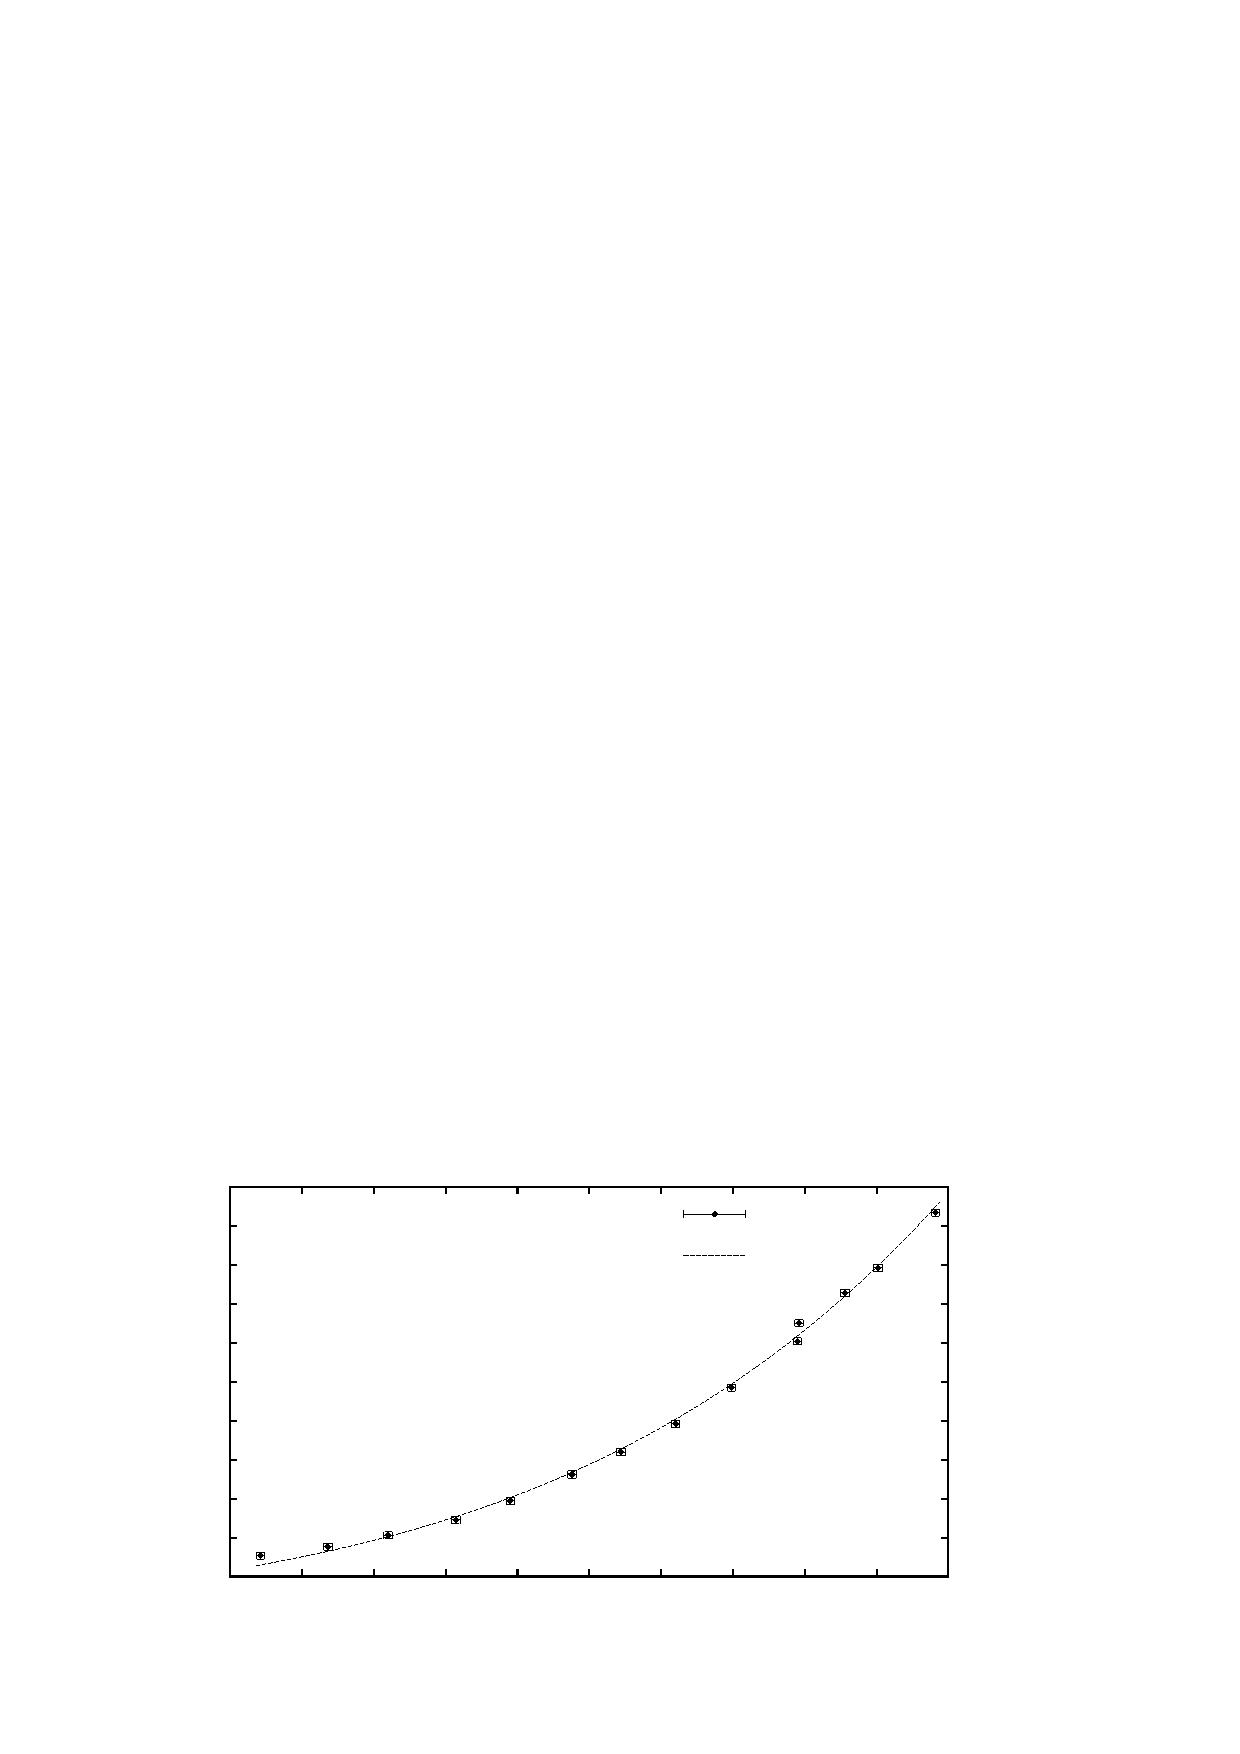
\includegraphics{pDk-T-diagram}}%
    \gplfronttext
  \end{picture}%
\endgroup

	\end{figure}

	\begin{figure}
		\center
		% GNUPLOT: LaTeX picture with Postscript
\begingroup
  \makeatletter
  \providecommand\color[2][]{%
    \GenericError{(gnuplot) \space\space\space\@spaces}{%
      Package color not loaded in conjunction with
      terminal option `colourtext'%
    }{See the gnuplot documentation for explanation.%
    }{Either use 'blacktext' in gnuplot or load the package
      color.sty in LaTeX.}%
    \renewcommand\color[2][]{}%
  }%
  \providecommand\includegraphics[2][]{%
    \GenericError{(gnuplot) \space\space\space\@spaces}{%
      Package graphicx or graphics not loaded%
    }{See the gnuplot documentation for explanation.%
    }{The gnuplot epslatex terminal needs graphicx.sty or graphics.sty.}%
    \renewcommand\includegraphics[2][]{}%
  }%
  \providecommand\rotatebox[2]{#2}%
  \@ifundefined{ifGPcolor}{%
    \newif\ifGPcolor
    \GPcolorfalse
  }{}%
  \@ifundefined{ifGPblacktext}{%
    \newif\ifGPblacktext
    \GPblacktexttrue
  }{}%
  % define a \g@addto@macro without @ in the name:
  \let\gplgaddtomacro\g@addto@macro
  % define empty templates for all commands taking text:
  \gdef\gplbacktext{}%
  \gdef\gplfronttext{}%
  \makeatother
  \ifGPblacktext
    % no textcolor at all
    \def\colorrgb#1{}%
    \def\colorgray#1{}%
  \else
    % gray or color?
    \ifGPcolor
      \def\colorrgb#1{\color[rgb]{#1}}%
      \def\colorgray#1{\color[gray]{#1}}%
      \expandafter\def\csname LTw\endcsname{\color{white}}%
      \expandafter\def\csname LTb\endcsname{\color{black}}%
      \expandafter\def\csname LTa\endcsname{\color{black}}%
      \expandafter\def\csname LT0\endcsname{\color[rgb]{1,0,0}}%
      \expandafter\def\csname LT1\endcsname{\color[rgb]{0,1,0}}%
      \expandafter\def\csname LT2\endcsname{\color[rgb]{0,0,1}}%
      \expandafter\def\csname LT3\endcsname{\color[rgb]{1,0,1}}%
      \expandafter\def\csname LT4\endcsname{\color[rgb]{0,1,1}}%
      \expandafter\def\csname LT5\endcsname{\color[rgb]{1,1,0}}%
      \expandafter\def\csname LT6\endcsname{\color[rgb]{0,0,0}}%
      \expandafter\def\csname LT7\endcsname{\color[rgb]{1,0.3,0}}%
      \expandafter\def\csname LT8\endcsname{\color[rgb]{0.5,0.5,0.5}}%
    \else
      % gray
      \def\colorrgb#1{\color{black}}%
      \def\colorgray#1{\color[gray]{#1}}%
      \expandafter\def\csname LTw\endcsname{\color{white}}%
      \expandafter\def\csname LTb\endcsname{\color{black}}%
      \expandafter\def\csname LTa\endcsname{\color{black}}%
      \expandafter\def\csname LT0\endcsname{\color{black}}%
      \expandafter\def\csname LT1\endcsname{\color{black}}%
      \expandafter\def\csname LT2\endcsname{\color{black}}%
      \expandafter\def\csname LT3\endcsname{\color{black}}%
      \expandafter\def\csname LT4\endcsname{\color{black}}%
      \expandafter\def\csname LT5\endcsname{\color{black}}%
      \expandafter\def\csname LT6\endcsname{\color{black}}%
      \expandafter\def\csname LT7\endcsname{\color{black}}%
      \expandafter\def\csname LT8\endcsname{\color{black}}%
    \fi
  \fi
  \setlength{\unitlength}{0.0500bp}%
  \begin{picture}(8502.00,5102.00)%
    \gplgaddtomacro\gplbacktext{%
      \csname LTb\endcsname%
      \put(814,704){\makebox(0,0)[r]{\strut{}4.5}}%
      \put(814,1451){\makebox(0,0)[r]{\strut{}5.0}}%
      \put(814,2199){\makebox(0,0)[r]{\strut{}5.5}}%
      \put(814,2946){\makebox(0,0)[r]{\strut{}6.0}}%
      \put(814,3694){\makebox(0,0)[r]{\strut{}6.5}}%
      \put(814,4441){\makebox(0,0)[r]{\strut{}7.0}}%
      \put(946,484){\makebox(0,0){\strut{}0.0028}}%
      \put(2139,484){\makebox(0,0){\strut{}0.0029}}%
      \put(3332,484){\makebox(0,0){\strut{}0.0030}}%
      \put(4525,484){\makebox(0,0){\strut{}0.0031}}%
      \put(5719,484){\makebox(0,0){\strut{}0.0032}}%
      \put(6912,484){\makebox(0,0){\strut{}0.0033}}%
      \put(8105,484){\makebox(0,0){\strut{}0.0034}}%
      \put(176,2572){\rotatebox{-270}{\makebox(0,0){\strut{}$\ln (p_D/p_0) \ [1]$}}}%
      \put(4525,154){\makebox(0,0){\strut{}$1/T \ [1/K]$}}%
      \put(4525,4771){\makebox(0,0){\strut{}Darstellung $\ln (p_D/p_0)$ über $1/T$ mit nicht korrigierten Werten und $p_0 = 1 \ Torr$}}%
      \put(4525,3694){\makebox(0,0)[l]{\strut{}$a\pm \Delta a = (-4621 \pm 84) \ K$}}%
      \put(4525,3395){\makebox(0,0)[l]{\strut{}$b\pm \Delta b = (20.26 \pm 0.25)$}}%
    }%
    \gplgaddtomacro\gplfronttext{%
      \csname LTb\endcsname%
      \put(7118,4268){\makebox(0,0)[r]{\strut{}Messwerte ohne Korrektur}}%
      \csname LTb\endcsname%
      \put(7118,4048){\makebox(0,0)[r]{\strut{}$f(x) = ax+b$}}%
    }%
    \gplbacktext
    \put(0,0){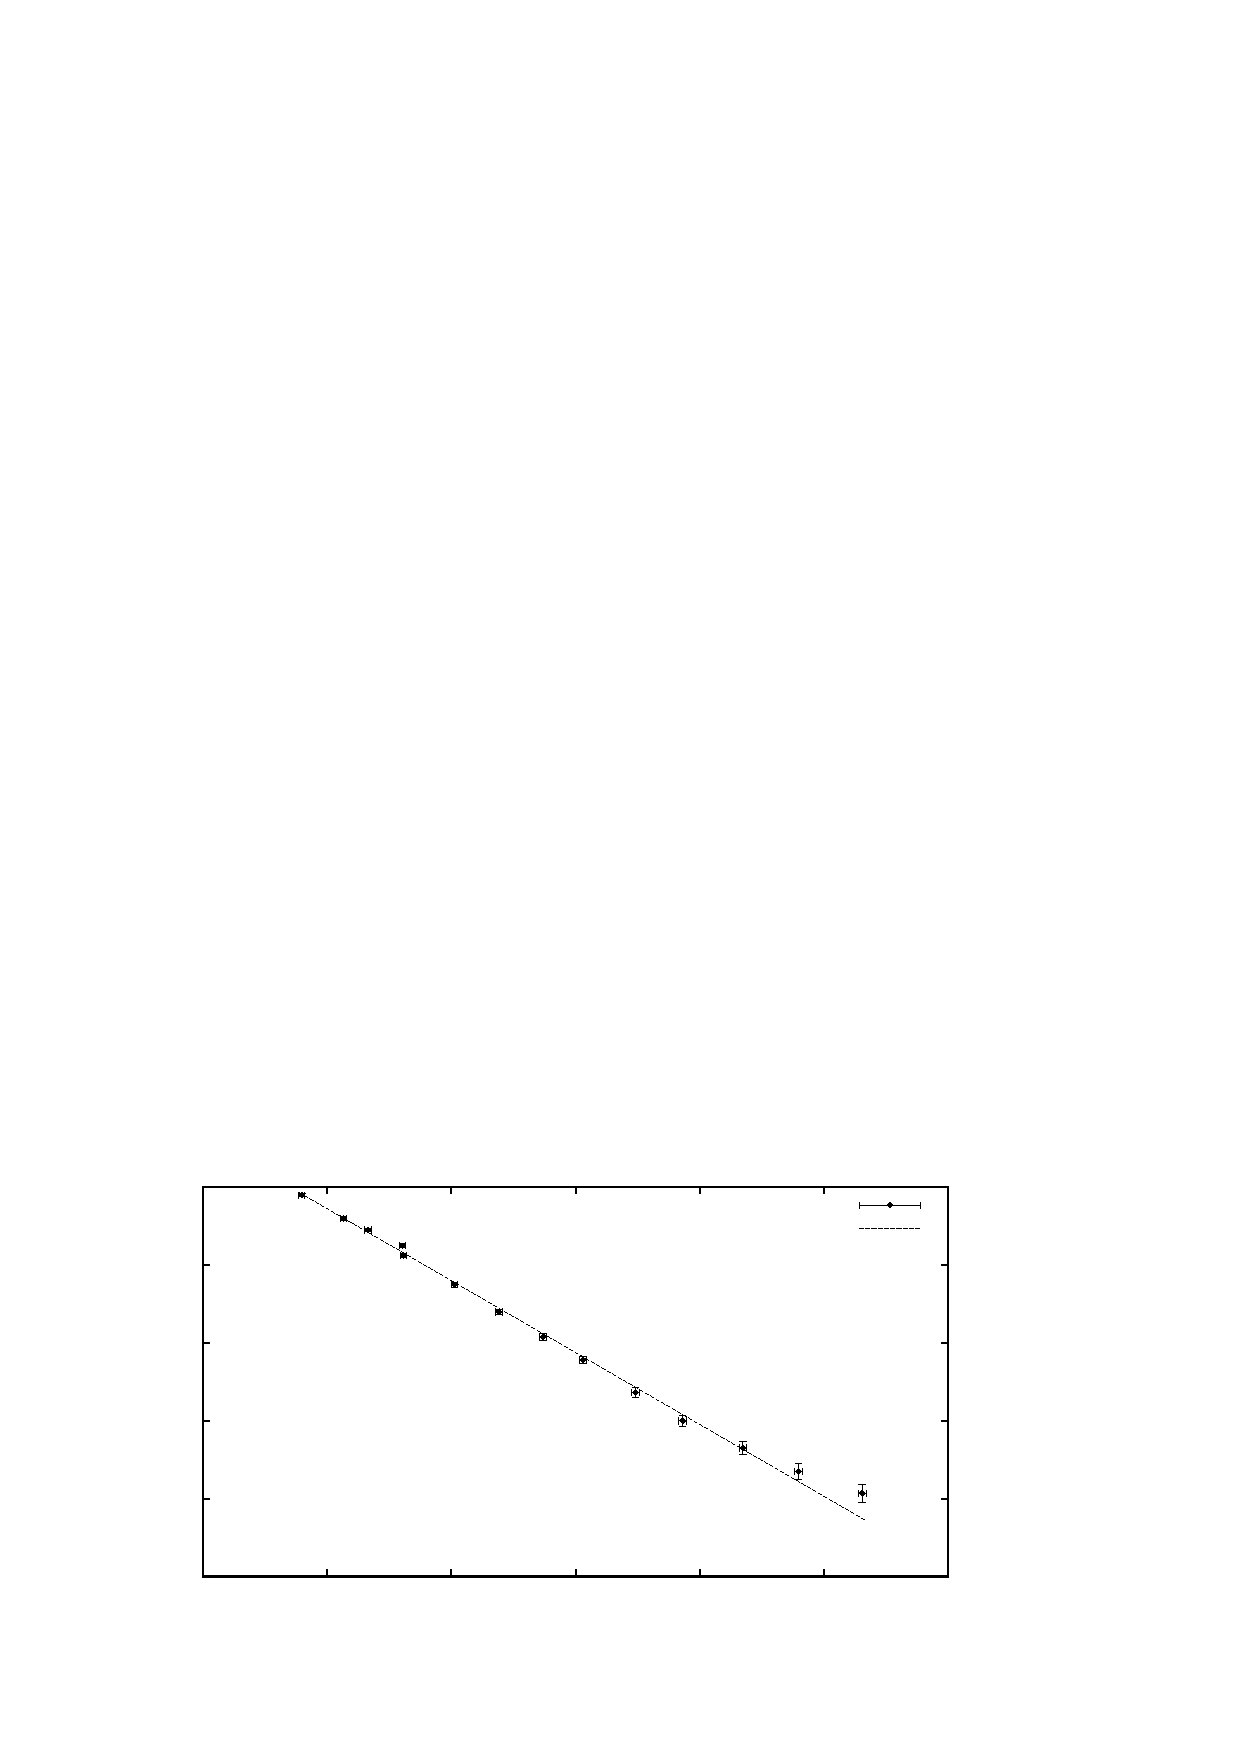
\includegraphics{Qv-diagram}}%
    \gplfronttext
  \end{picture}%
\endgroup

	\end{figure}

	\begin{figure}
		\center
		% GNUPLOT: LaTeX picture with Postscript
\begingroup
  \makeatletter
  \providecommand\color[2][]{%
    \GenericError{(gnuplot) \space\space\space\@spaces}{%
      Package color not loaded in conjunction with
      terminal option `colourtext'%
    }{See the gnuplot documentation for explanation.%
    }{Either use 'blacktext' in gnuplot or load the package
      color.sty in LaTeX.}%
    \renewcommand\color[2][]{}%
  }%
  \providecommand\includegraphics[2][]{%
    \GenericError{(gnuplot) \space\space\space\@spaces}{%
      Package graphicx or graphics not loaded%
    }{See the gnuplot documentation for explanation.%
    }{The gnuplot epslatex terminal needs graphicx.sty or graphics.sty.}%
    \renewcommand\includegraphics[2][]{}%
  }%
  \providecommand\rotatebox[2]{#2}%
  \@ifundefined{ifGPcolor}{%
    \newif\ifGPcolor
    \GPcolorfalse
  }{}%
  \@ifundefined{ifGPblacktext}{%
    \newif\ifGPblacktext
    \GPblacktexttrue
  }{}%
  % define a \g@addto@macro without @ in the name:
  \let\gplgaddtomacro\g@addto@macro
  % define empty templates for all commands taking text:
  \gdef\gplbacktext{}%
  \gdef\gplfronttext{}%
  \makeatother
  \ifGPblacktext
    % no textcolor at all
    \def\colorrgb#1{}%
    \def\colorgray#1{}%
  \else
    % gray or color?
    \ifGPcolor
      \def\colorrgb#1{\color[rgb]{#1}}%
      \def\colorgray#1{\color[gray]{#1}}%
      \expandafter\def\csname LTw\endcsname{\color{white}}%
      \expandafter\def\csname LTb\endcsname{\color{black}}%
      \expandafter\def\csname LTa\endcsname{\color{black}}%
      \expandafter\def\csname LT0\endcsname{\color[rgb]{1,0,0}}%
      \expandafter\def\csname LT1\endcsname{\color[rgb]{0,1,0}}%
      \expandafter\def\csname LT2\endcsname{\color[rgb]{0,0,1}}%
      \expandafter\def\csname LT3\endcsname{\color[rgb]{1,0,1}}%
      \expandafter\def\csname LT4\endcsname{\color[rgb]{0,1,1}}%
      \expandafter\def\csname LT5\endcsname{\color[rgb]{1,1,0}}%
      \expandafter\def\csname LT6\endcsname{\color[rgb]{0,0,0}}%
      \expandafter\def\csname LT7\endcsname{\color[rgb]{1,0.3,0}}%
      \expandafter\def\csname LT8\endcsname{\color[rgb]{0.5,0.5,0.5}}%
    \else
      % gray
      \def\colorrgb#1{\color{black}}%
      \def\colorgray#1{\color[gray]{#1}}%
      \expandafter\def\csname LTw\endcsname{\color{white}}%
      \expandafter\def\csname LTb\endcsname{\color{black}}%
      \expandafter\def\csname LTa\endcsname{\color{black}}%
      \expandafter\def\csname LT0\endcsname{\color{black}}%
      \expandafter\def\csname LT1\endcsname{\color{black}}%
      \expandafter\def\csname LT2\endcsname{\color{black}}%
      \expandafter\def\csname LT3\endcsname{\color{black}}%
      \expandafter\def\csname LT4\endcsname{\color{black}}%
      \expandafter\def\csname LT5\endcsname{\color{black}}%
      \expandafter\def\csname LT6\endcsname{\color{black}}%
      \expandafter\def\csname LT7\endcsname{\color{black}}%
      \expandafter\def\csname LT8\endcsname{\color{black}}%
    \fi
  \fi
  \setlength{\unitlength}{0.0500bp}%
  \begin{picture}(8502.00,5102.00)%
    \gplgaddtomacro\gplbacktext{%
      \csname LTb\endcsname%
      \put(814,704){\makebox(0,0)[r]{\strut{}4.5}}%
      \put(814,1451){\makebox(0,0)[r]{\strut{}5.0}}%
      \put(814,2199){\makebox(0,0)[r]{\strut{}5.5}}%
      \put(814,2946){\makebox(0,0)[r]{\strut{}6.0}}%
      \put(814,3694){\makebox(0,0)[r]{\strut{}6.5}}%
      \put(814,4441){\makebox(0,0)[r]{\strut{}7.0}}%
      \put(946,484){\makebox(0,0){\strut{}0.0028}}%
      \put(2139,484){\makebox(0,0){\strut{}0.0029}}%
      \put(3332,484){\makebox(0,0){\strut{}0.0030}}%
      \put(4525,484){\makebox(0,0){\strut{}0.0031}}%
      \put(5719,484){\makebox(0,0){\strut{}0.0032}}%
      \put(6912,484){\makebox(0,0){\strut{}0.0033}}%
      \put(8105,484){\makebox(0,0){\strut{}0.0034}}%
      \put(176,2572){\rotatebox{-270}{\makebox(0,0){\strut{}$\ln (p_D/p_0) \ [1]$}}}%
      \put(4525,154){\makebox(0,0){\strut{}$1/T \ [1/K]$}}%
      \put(4525,4771){\makebox(0,0){\strut{}Darstellung $\ln (p_{D_0}/p_0)$ über $1/T$ mit korrigierten Werten und $p_0 = 1 \ Torr$}}%
      \put(4525,3694){\makebox(0,0)[l]{\strut{}$a\pm \Delta a = (-4593 \pm 82) \ K$}}%
      \put(4525,3395){\makebox(0,0)[l]{\strut{}$b\pm \Delta b = (20.18 \pm 0.24)$}}%
    }%
    \gplgaddtomacro\gplfronttext{%
      \csname LTb\endcsname%
      \put(7118,4268){\makebox(0,0)[r]{\strut{}Messwerte mit Korrektur}}%
      \csname LTb\endcsname%
      \put(7118,4048){\makebox(0,0)[r]{\strut{}$f(x) = ax+b$}}%
    }%
    \gplbacktext
    \put(0,0){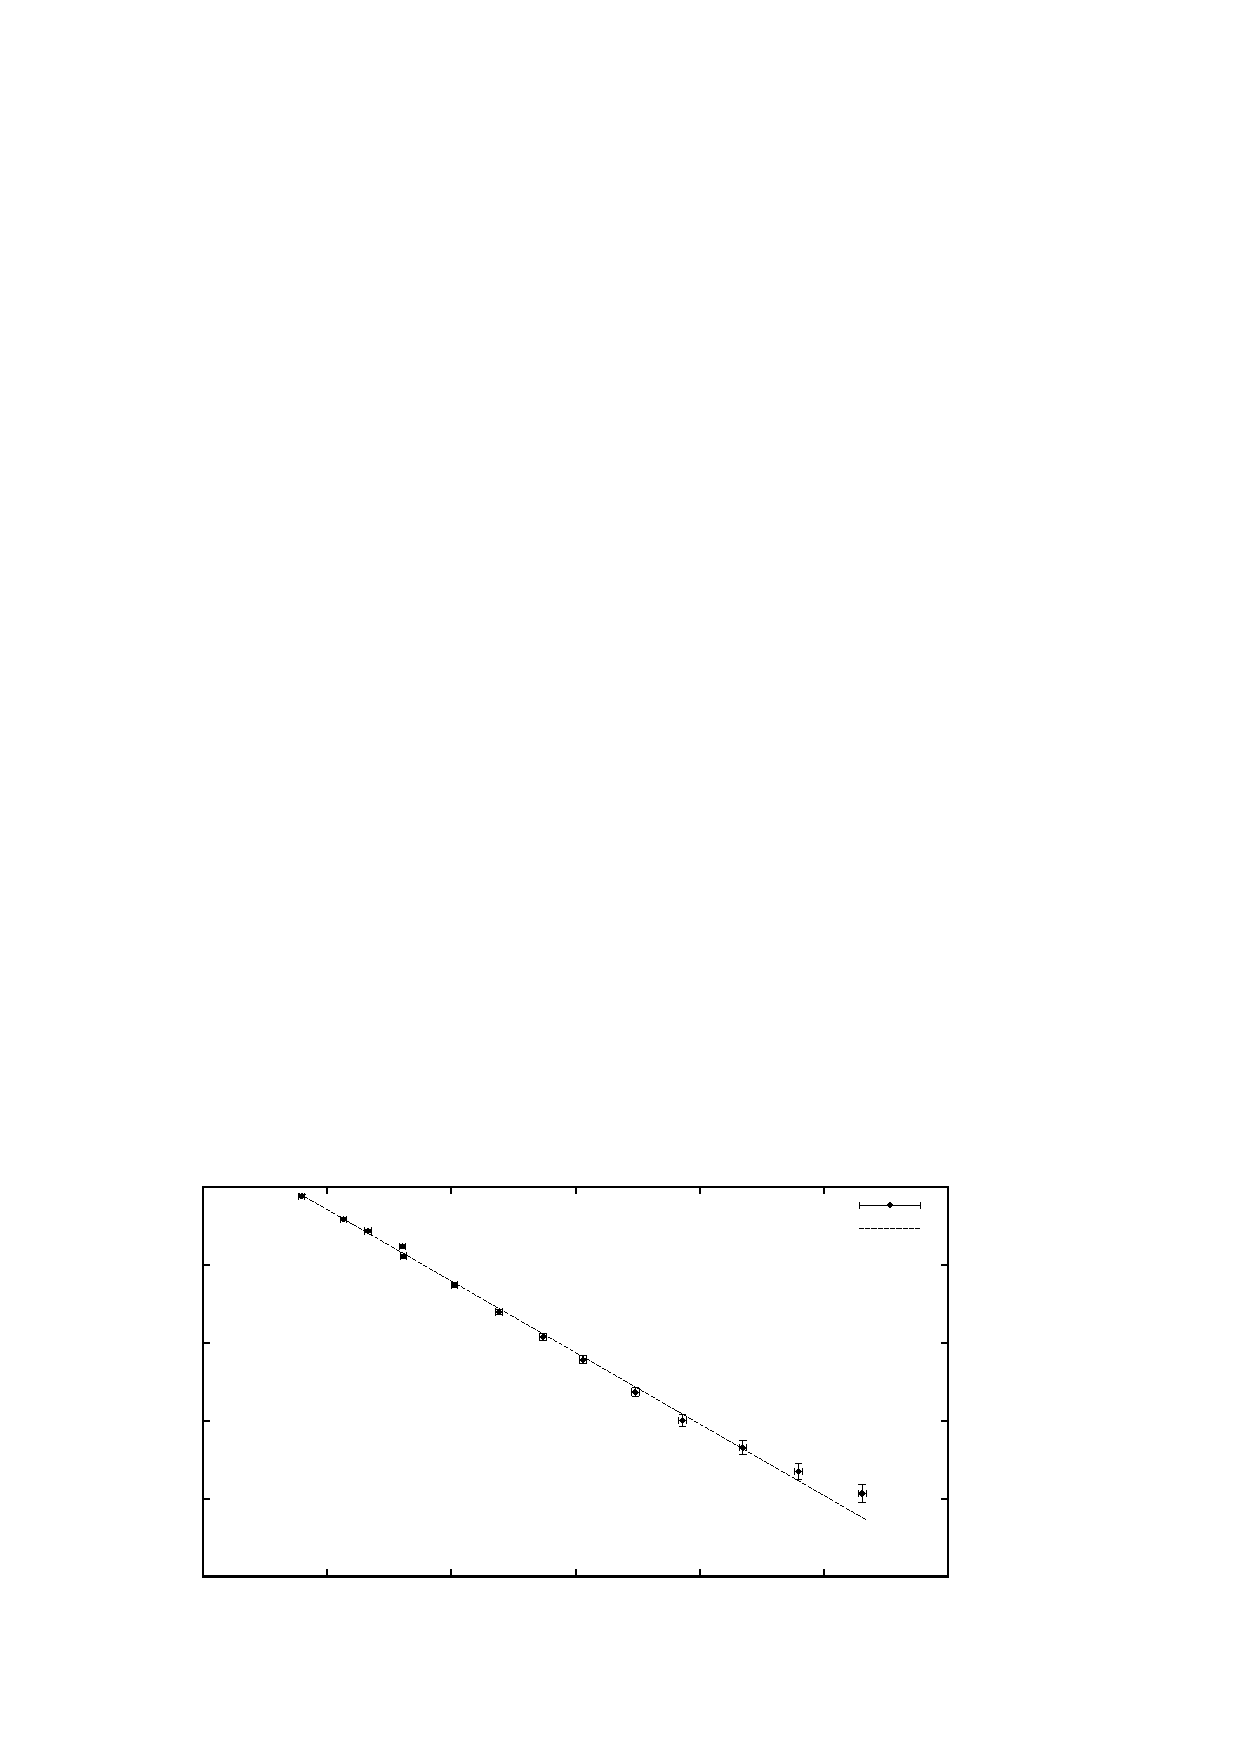
\includegraphics{Qvk-diagram}}%
    \gplfronttext
  \end{picture}%
\endgroup

	\end{figure}

	\begin{figure}
		\center
		% GNUPLOT: LaTeX picture with Postscript
\begingroup
  \makeatletter
  \providecommand\color[2][]{%
    \GenericError{(gnuplot) \space\space\space\@spaces}{%
      Package color not loaded in conjunction with
      terminal option `colourtext'%
    }{See the gnuplot documentation for explanation.%
    }{Either use 'blacktext' in gnuplot or load the package
      color.sty in LaTeX.}%
    \renewcommand\color[2][]{}%
  }%
  \providecommand\includegraphics[2][]{%
    \GenericError{(gnuplot) \space\space\space\@spaces}{%
      Package graphicx or graphics not loaded%
    }{See the gnuplot documentation for explanation.%
    }{The gnuplot epslatex terminal needs graphicx.sty or graphics.sty.}%
    \renewcommand\includegraphics[2][]{}%
  }%
  \providecommand\rotatebox[2]{#2}%
  \@ifundefined{ifGPcolor}{%
    \newif\ifGPcolor
    \GPcolorfalse
  }{}%
  \@ifundefined{ifGPblacktext}{%
    \newif\ifGPblacktext
    \GPblacktexttrue
  }{}%
  % define a \g@addto@macro without @ in the name:
  \let\gplgaddtomacro\g@addto@macro
  % define empty templates for all commands taking text:
  \gdef\gplbacktext{}%
  \gdef\gplfronttext{}%
  \makeatother
  \ifGPblacktext
    % no textcolor at all
    \def\colorrgb#1{}%
    \def\colorgray#1{}%
  \else
    % gray or color?
    \ifGPcolor
      \def\colorrgb#1{\color[rgb]{#1}}%
      \def\colorgray#1{\color[gray]{#1}}%
      \expandafter\def\csname LTw\endcsname{\color{white}}%
      \expandafter\def\csname LTb\endcsname{\color{black}}%
      \expandafter\def\csname LTa\endcsname{\color{black}}%
      \expandafter\def\csname LT0\endcsname{\color[rgb]{1,0,0}}%
      \expandafter\def\csname LT1\endcsname{\color[rgb]{0,1,0}}%
      \expandafter\def\csname LT2\endcsname{\color[rgb]{0,0,1}}%
      \expandafter\def\csname LT3\endcsname{\color[rgb]{1,0,1}}%
      \expandafter\def\csname LT4\endcsname{\color[rgb]{0,1,1}}%
      \expandafter\def\csname LT5\endcsname{\color[rgb]{1,1,0}}%
      \expandafter\def\csname LT6\endcsname{\color[rgb]{0,0,0}}%
      \expandafter\def\csname LT7\endcsname{\color[rgb]{1,0.3,0}}%
      \expandafter\def\csname LT8\endcsname{\color[rgb]{0.5,0.5,0.5}}%
    \else
      % gray
      \def\colorrgb#1{\color{black}}%
      \def\colorgray#1{\color[gray]{#1}}%
      \expandafter\def\csname LTw\endcsname{\color{white}}%
      \expandafter\def\csname LTb\endcsname{\color{black}}%
      \expandafter\def\csname LTa\endcsname{\color{black}}%
      \expandafter\def\csname LT0\endcsname{\color{black}}%
      \expandafter\def\csname LT1\endcsname{\color{black}}%
      \expandafter\def\csname LT2\endcsname{\color{black}}%
      \expandafter\def\csname LT3\endcsname{\color{black}}%
      \expandafter\def\csname LT4\endcsname{\color{black}}%
      \expandafter\def\csname LT5\endcsname{\color{black}}%
      \expandafter\def\csname LT6\endcsname{\color{black}}%
      \expandafter\def\csname LT7\endcsname{\color{black}}%
      \expandafter\def\csname LT8\endcsname{\color{black}}%
    \fi
  \fi
  \setlength{\unitlength}{0.0500bp}%
  \begin{picture}(8502.00,5102.00)%
    \gplgaddtomacro\gplbacktext{%
      \csname LTb\endcsname%
      \put(814,704){\makebox(0,0)[r]{\strut{}5.0}}%
      \put(814,1044){\makebox(0,0)[r]{\strut{}5.2}}%
      \put(814,1383){\makebox(0,0)[r]{\strut{}5.4}}%
      \put(814,1723){\makebox(0,0)[r]{\strut{}5.6}}%
      \put(814,2063){\makebox(0,0)[r]{\strut{}5.8}}%
      \put(814,2403){\makebox(0,0)[r]{\strut{}6.0}}%
      \put(814,2742){\makebox(0,0)[r]{\strut{}6.2}}%
      \put(814,3082){\makebox(0,0)[r]{\strut{}6.4}}%
      \put(814,3422){\makebox(0,0)[r]{\strut{}6.6}}%
      \put(814,3762){\makebox(0,0)[r]{\strut{}6.8}}%
      \put(814,4101){\makebox(0,0)[r]{\strut{}7.0}}%
      \put(814,4441){\makebox(0,0)[r]{\strut{}7.2}}%
      \put(946,484){\makebox(0,0){\strut{}0.0028}}%
      \put(2139,484){\makebox(0,0){\strut{}0.0029}}%
      \put(3332,484){\makebox(0,0){\strut{}0.0030}}%
      \put(4525,484){\makebox(0,0){\strut{}0.0031}}%
      \put(5719,484){\makebox(0,0){\strut{}0.0032}}%
      \put(6912,484){\makebox(0,0){\strut{}0.0033}}%
      \put(8105,484){\makebox(0,0){\strut{}0.0034}}%
      \put(176,2572){\rotatebox{-270}{\makebox(0,0){\strut{}$\ln (p_D/p_0) \ [1]$}}}%
      \put(4525,154){\makebox(0,0){\strut{}$1/T \ [1/K]$}}%
      \put(4525,4771){\makebox(0,0){\strut{}Darstellung $\ln (p_D/p_0)$ über $1/T$ mit korrigierten systematischen Fehler und $p_0 = 1 \ Torr$}}%
      \put(4525,3252){\makebox(0,0)[l]{\strut{}$a\pm \Delta a = (-4177 \pm 96) \ K$}}%
      \put(4525,2912){\makebox(0,0)[l]{\strut{}$b\pm \Delta b = (19.00 \pm 0.28)$}}%
    }%
    \gplgaddtomacro\gplfronttext{%
      \csname LTb\endcsname%
      \put(7118,4268){\makebox(0,0)[r]{\strut{}Messwerte ohne Korrektur}}%
      \csname LTb\endcsname%
      \put(7118,4048){\makebox(0,0)[r]{\strut{}$f(x) = ax+b$}}%
    }%
    \gplbacktext
    \put(0,0){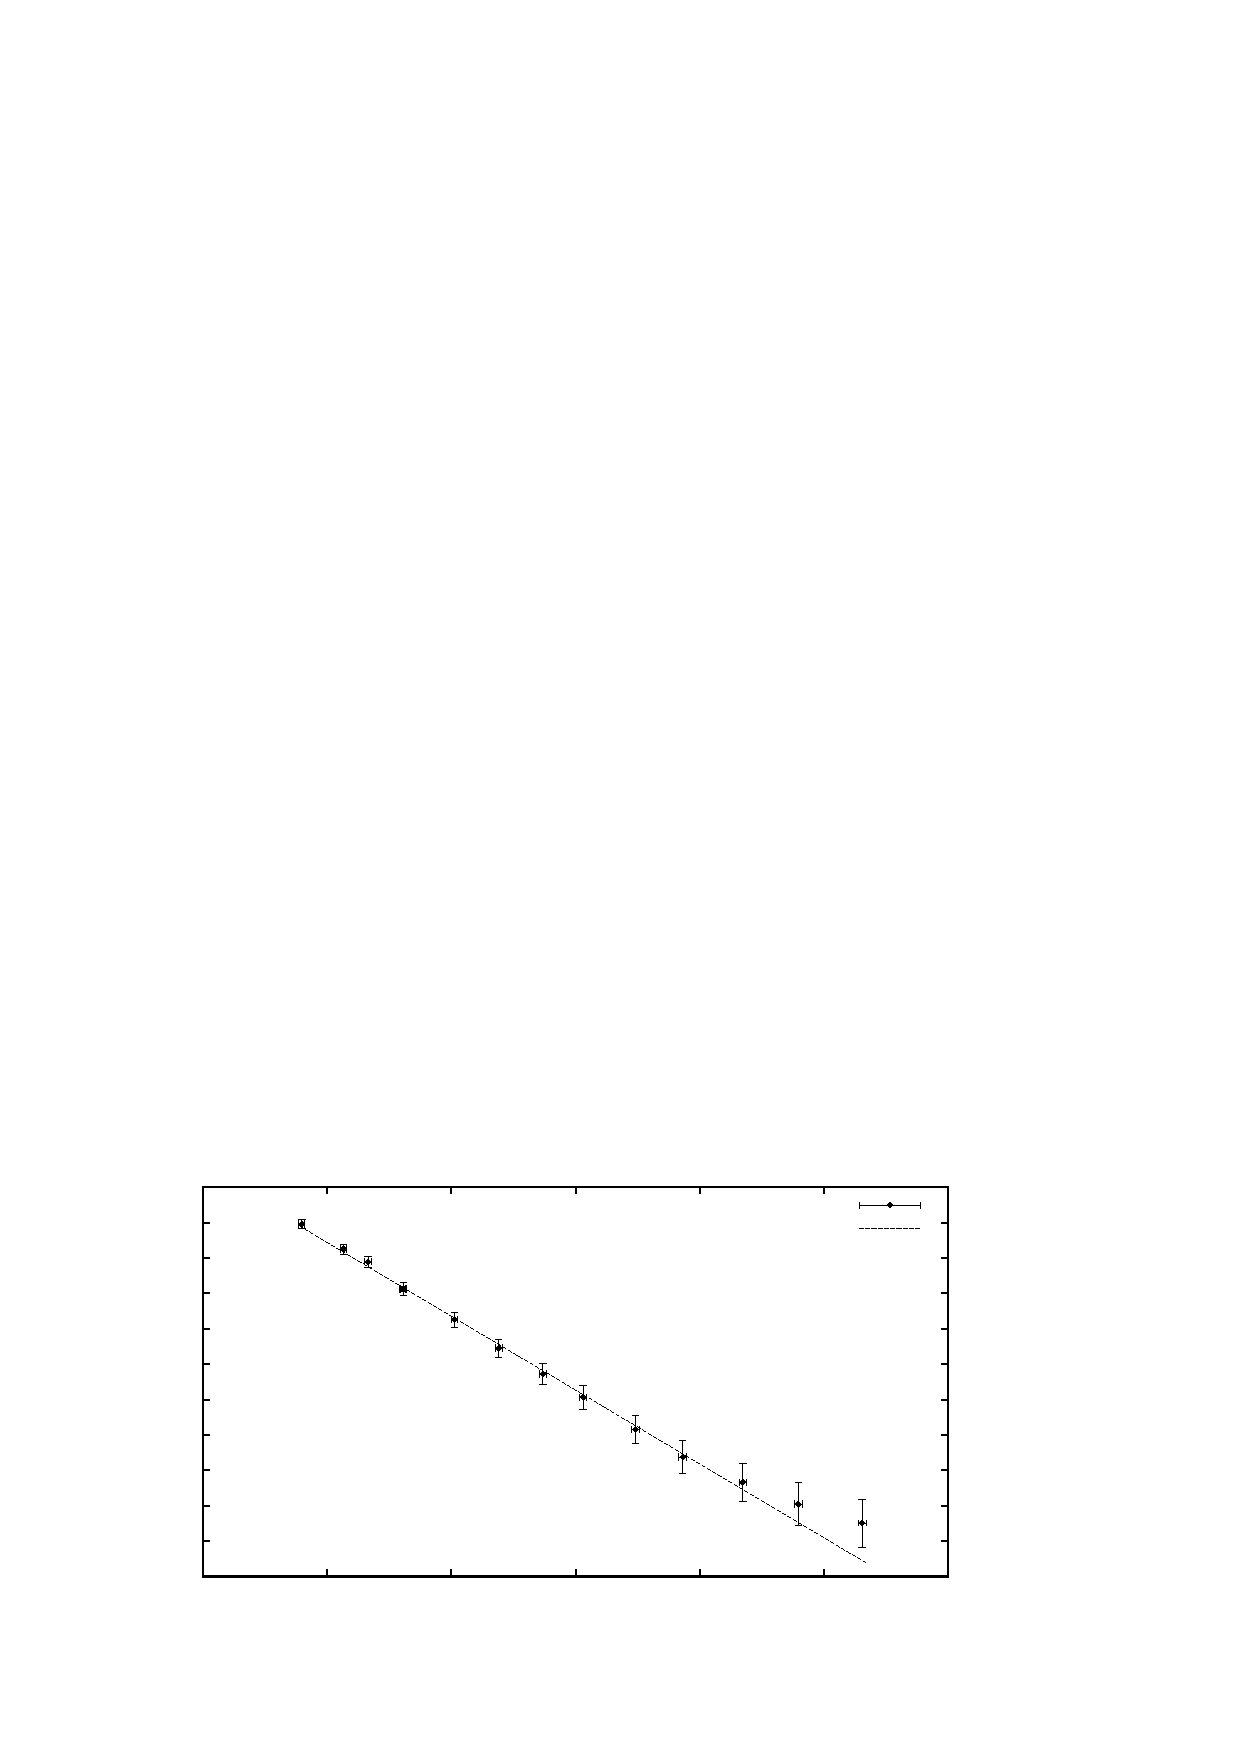
\includegraphics{Qvk2-diagram}}%
    \gplfronttext
  \end{picture}%
\endgroup

	\end{figure}

\end{document}

